\chapter{Einf\"uhrung und \"Uberblick}
\label{chp:Intro}
Dieses Kapitel f\"uhrt in \ldots\ ein. Dies ist \zB\ eine Referenz: \cite{Prieur2009}. Dazu ist ein separates BibTeX-File erforderlich.

\section{Bilder und Allgemeines}
\label{sec:1:BilderUndSo}
In Abbildung~\ref{fig:bibtex} ist die zu dieser Vorlage geh\"orende Literaturdatenbank (BibTeX) zu sehen.

\begin{figure}[htbp]
	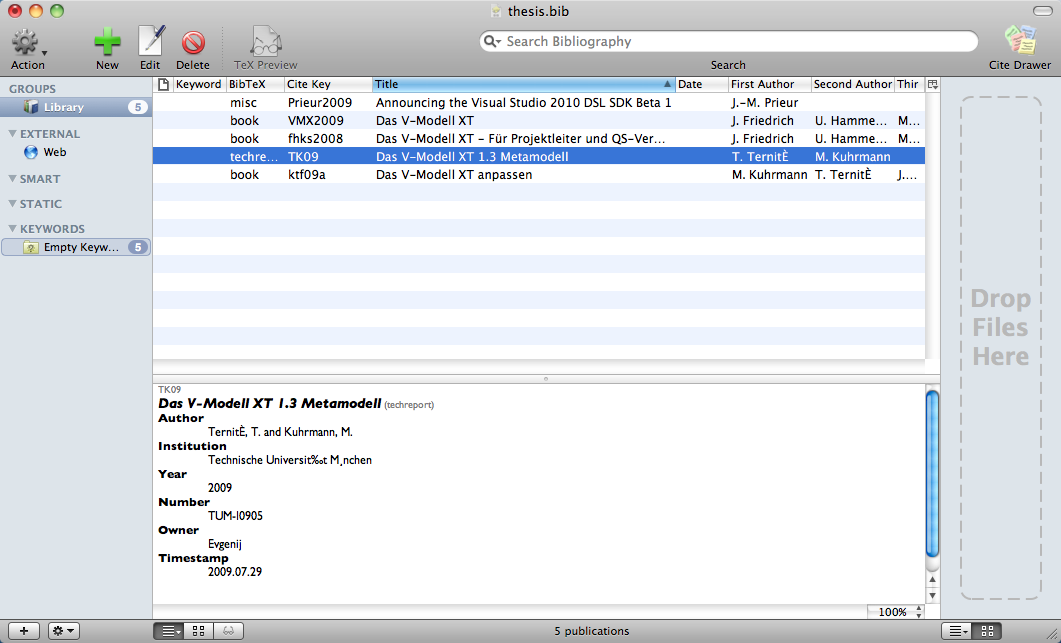
\includegraphics[width=1.00\textwidth]{imgs/bibtex.png}
	\caption{BibTeX-File f\"ur diese Vorlage}
	\label{fig:bibtex}
\end{figure}

Nebenbei zeigt der letzte Abschnitt gleichzeitig, wie eine Abbildung in die Arbeit eingebunden wird. Eine Skalierung dieses Bildes, \zB\ auf die halbe Breite des Textes und zentriert sieht dann so aus, wie in Abbildung~\ref{fig:bibtex2} dargestellt.

\begin{figure}[htbp]
	\centering
	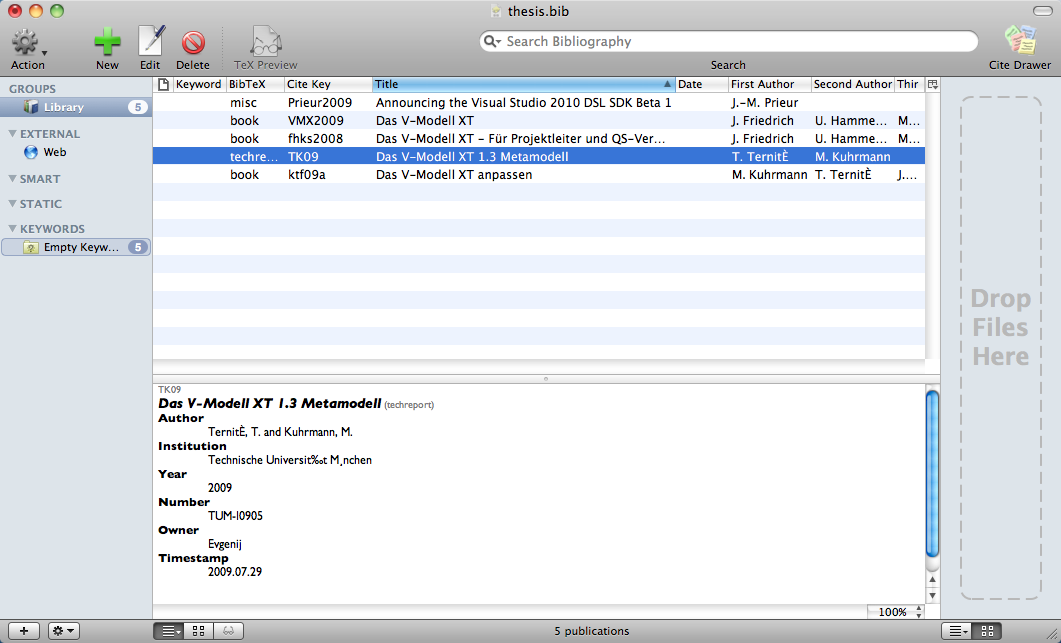
\includegraphics[width=0.5\textwidth]{imgs/bibtex.png}
	\caption[Alternativtext]{BibTeX-File f\"ur diese Vorlage -- nun in Klein}
	\label{fig:bibtex2}
\end{figure}

\begin{MySugg}
	Zu beachten ist bei Abbildungen als grobe Richtschnur: Das gr\"o{\ss}te Zeichen in der Abbildung sollte nicht gr\"o{\ss}er erscheinen, als das gro{\ss}e \emph{A} im ,,Abbildung'' der Bildunterschrift.
\end{MySugg}

Nebenbei war gerade zu sehen, wie ein spezielle Umgebung f\"ur Hinweise im Flie{\ss}text aussieht. Zur Anwendung kommt die Umgebung \kw{MySugg}, die in der Datei \kw{commands.tex} definiert ist. Ebenso gibt es dort die Umgebungen \kw{MySample} und \kw{MyBox}. Diese und die anderen Definitionen in der Datei helfen, viele Aufgaben etwas zu vereinfachen und die Ausgaben etwas aufzuh\"ubschen.

Weiterhin treten recht h\"aufig Aufz\"ahlungen und Listen auf. In dieser Vorlage ist das Paket \emph{paralist} eingebunden, das die Umgebungen \kw{compactitem} und \kw{compactenum} enth\"alt. Ein Beipiel f\"ur eine ,,klassische'' Liste ist:

\begin{itemize}
	\item Item 1
	\item Item 2
	\item Item 3
\end{itemize}

Mit der neuen Umgebung wird nicht mehr soviel Platz verschwendet, weshalb wir diese empfehlen:


\begin{compactitem}
	\item Item 1
	\item Item 2
	\item Item 3
\end{compactitem}


\section{Tabellen}
\label{sec:Tabellen}
Und so sehen die ,,h\"ubschen'' Tabellen aus\ldots

\begin{table}[htbp]
\begin{tabularx}
	{\linewidth}{@{}!{\color{white}\vrule}>{\hspace{0mm}}lL<{\hspace{0mm}} !{\color{white}\vrule width 0pt}@{}}
	\opentableheader	%\toprule
		\hl{Element} & \hl{Beschreibung} \\
	\closetableheader %\endtabularhead
		Element & Beschreibung \\
		Element & Beschreibung \\
		\midrule
		Element & Beschreibung, Beschreibung, Beschreibung, Beschreibung, Beschreibung, Beschreibung, Beschreibung, Beschreibung, Beschreibung, Beschreibung, Beschreibung\ldots \\
	\bottomrule
\end{tabularx}
  \caption[Alternativtext f\"ur das Verzeichnis]{Beispiel: Beispiel f\"ur typographisch ,,bessere'' Tabellen}%
  \label{tab:BeschreibungAllgemeinesNamensschema}
\end{table}

\begin{table}[!ht]
\begin{center}
\begin{tabular} {ll}
	\opentableheader	%\toprule
		\hl{Element} & \hl{Beschreibung} \\
	\closetableheader %\endtabularhead
		Element & Beschreibung \\
		Element & Beschreibung \\
		\midrule
		Element & Beschreibung \\
	\bottomrule
\end{tabular}
\end{center}
  \caption{Beispiel: Nicht skalierte Tabelle}%
  \label{tab:TabUnskaliert}
\end{table}

Das gro{\ss}e \emph{L} in Tabelle~\ref{tab:BeschreibungAllgemeinesNamensschema} (vgl.\ Listing~\ref{lst:TabellenCode}) sorgt daf\"ur, dass die Tabelle \"uber die gesamte Textbreite (nicht mehr und nicht weniger) skaliert. Es sogt gleichzeitig daf\"ur, dass ein automatischer Zeilenumbruch durchgef\"uhrt wird.

\begin{lstlisting}[captionpos=b, caption=Listing f\"ur die oben stehende Tabelle,label=lst:TabellenCode]
\begin{table}[htbp]
\begin{tabularx}
  {\linewidth}{@{}!{\color{white}\vrule}>{\hspace{0mm}}lL<{\hspace{0mm}} !{\color{white}\vrule width 0pt}@{}}
  \opentableheader	%\toprule
	\hl{Element} & \hl{Beschreibung} \\
  \closetableheader %\endtabularhead
	Element & Beschreibung \\
	Element & Beschreibung \\
	\midrule
	Element & Beschreibung \\
  \bottomrule
\end{tabularx}
  \caption[Alternativtext f\"ur das Verzeichnis]{Beispiel: Beispiel f\"ur typographisch ,,bessere'' Tabellen}%
  \label{tab:BeschreibungAllgemeinesNamensschema}
\end{table}
\end{lstlisting}

Soll die Tabelle~\ref{tab:BeschreibungAllgemeinesNamensschema} nicht \"uber die Seitenbreite skalieren, muss das gro{\ss}e L gegen das \"ubliche, kleine getauscht werden und es kann die ,,normale'' Umgebung \kw{table} verwendet werden. Das Aussehen zeigt die Tabelle~\ref{tab:TabUnskaliert}.

\section{Listings}
\label{sec:2:Listings}
Das Listing~\ref{lst:TabellenCode} zeigt gleichzeitig auch, wie Codefragmente mithilfe des \emph{Listings}-Paket eingebunden werden. In der Datei \kw{commands.tex} gibt es daf\"ur auch einige Makros und Hilfen, um den Umgang mit dem Paket etwas zu vereinfachen...


%%% Local Variables:
%%% mode: latex
%%% TeX-master: "thesis"
%%% End:
